\subsection{ML Model Performance Measures}\label{subsec:misc_measures}

\onehalfspacing

\begin{verbatim}
INFO - PyTorch LR: learning_rate=0.01,
    epochs=10000 (SYS, DIA, MAP from 34 Median PPG Features)
    MSE: 217.2289, RMSE: 14.7387, MAE: 11.091,
    R^2: 0.062, Bias: -0.012, LoA: (-28.902, 28.877)
\end{verbatim}

\begin{verbatim}
INFO - PyTorch LR (WA): learning_rate=0.01,
    epochs=10000 (SYS, DIA, MAP from 34 Median PPG Features)
    MSE: 217.2582, RMSE: 14.7397, MAE: 11.093,
    R^2: 0.063, Bias: -0.019, LoA: (-28.910, 28.873)
\end{verbatim}

\begin{verbatim}
INFO - PyTorch MLP: learning_rate=0.01,
    epochs=10000 (SYS, DIA, MAP from 34 Median PPG Features)
    MSE: 196.1354, RMSE: 14.0048, MAE: 10.567,
    R^2: 0.152, Bias: 0.046, LoA: (-27.405, 27.497)
\end{verbatim}

\begin{verbatim}
INFO - PyTorch MLP (WA): learning_rate=0.01,
    epochs=10000 (SYS, DIA, MAP from 34 Median PPG Features)
    MSE: 249.7456, RMSE: 15.8033, MAE: 11.802,
    R^2: -0.072, Bias: -1.373, LoA: (-32.233, 29.486)
\end{verbatim}

\begin{verbatim}
INFO - PyTorch LSTM: learning_rate=0.1,
    epochs=100 (SYS, DIA, MAP from 34 Median PPG Features)
    MSE: 101.4742, RMSE: 10.0734, MAE: 7.119,
    R^2: 0.556, Bias: -0.034, LoA: (-19.779, 19.711)
\end{verbatim}

\begin{verbatim}
INFO - PyTorch LSTM (WA): learning_rate=0.1,
    epochs=100 (SYS, DIA, MAP from 34 Median PPG Features)
    MSE: 143.2955, RMSE: 11.9706, MAE: 8.697,
    R^2: 0.373, Bias: 0.056, LoA: (-23.408, 23.520)
\end{verbatim}

\begin{verbatim}
INFO - PyTorch Bi-LSTM: learning_rate=0.1,
    epochs=100 (SYS, DIA, MAP from 34 Median PPG Features)
    MSE: 118.1035, RMSE: 10.8675, MAE: 7.850,
    R^2: 0.481, Bias: 0.114, LoA: (-21.187, 21.414)
\end{verbatim}

\begin{verbatim}
INFO - PyTorch Bi-LSTM (WA): learning_rate=0.1,
    epochs=100 (SYS, DIA, MAP from 34 Median PPG Features)
    MSE: 159.7223, RMSE: 12.6381, MAE: 9.362,
    R^2: 0.303, Bias: -0.005, LoA: (-24.778, 24.767)
\end{verbatim}

\begin{verbatim}
INFO - PyTorch GRU: learning_rate=0.1,
    epochs=100 (SYS, DIA, MAP from 34 Median PPG Features)
    MSE: 93.5903, RMSE: 9.6742, MAE: 6.823,
    R^2: 0.587, Bias: -0.034, LoA: (-18.997, 18.928)
\end{verbatim}

\begin{verbatim}
INFO - PyTorch GRU (WA): learning_rate=0.1,
    epochs=100 (SYS, DIA, MAP from 34 Median PPG Features)
    MSE: 142.1063, RMSE: 11.9208, MAE: 8.658,
    R^2: 0.377, Bias: -0.059, LoA: (-23.425, 23.308)
\end{verbatim}

\begin{verbatim}
INFO - PyTorch Bi-GRU: learning_rate=0.1,
    epochs=100 (SYS, DIA, MAP from 34 Median PPG Features)
    MSE: 117.7146, RMSE: 10.8496, MAE: 7.844,
    R^2: 0.482, Bias: 0.034, LoA: (-21.233, 21.300)
\end{verbatim}

\begin{verbatim}
INFO - PyTorch Bi-GRU (WA): learning_rate=0.1,
    epochs=100 (SYS, DIA, MAP from 34 Median PPG Features)
    MSE: 173.8695, RMSE: 13.1860, MAE: 9.811,
    R^2: 0.241, Bias: -0.087, LoA: (-25.933, 25.759)
\end{verbatim}

\begin{verbatim}
INFO - RF (SYS, DIA, MAP from 34 Median PPG Features)
    MSE: 66.383, MAE: 5.075,
    R^2: 0.713, Bias: 0.069,
    LoA: [16.037, 16.037]
\end{verbatim}

\newpage

\subsection{Feature Importance Plots}\label{subsec:plots_fi}

\begin{figure}[b!]
    \centering
    \hspace{-2cm}
    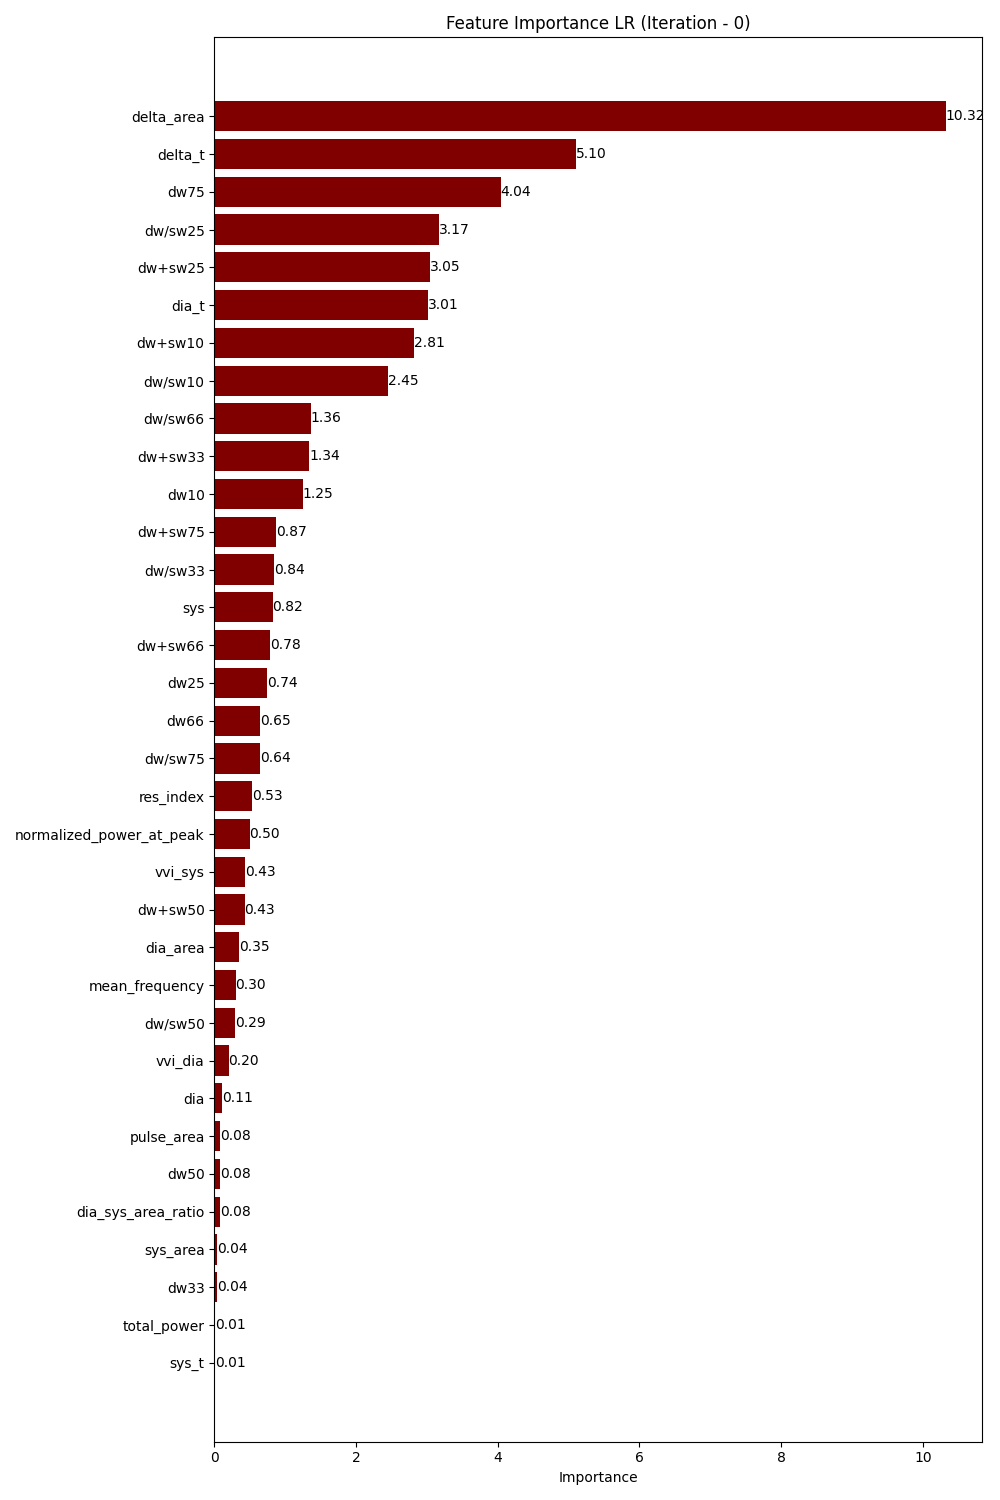
\includegraphics[width=0.82\textwidth]{images/results/feature_importance/feature_importance_plot_LR_0}
    \caption{Feature Importance Chart LR}
    \label{fig:fi_lr}
\end{figure}

\begin{figure}[h]
    \centering
    \vspace{-1cm}
    \hspace{-2cm}
    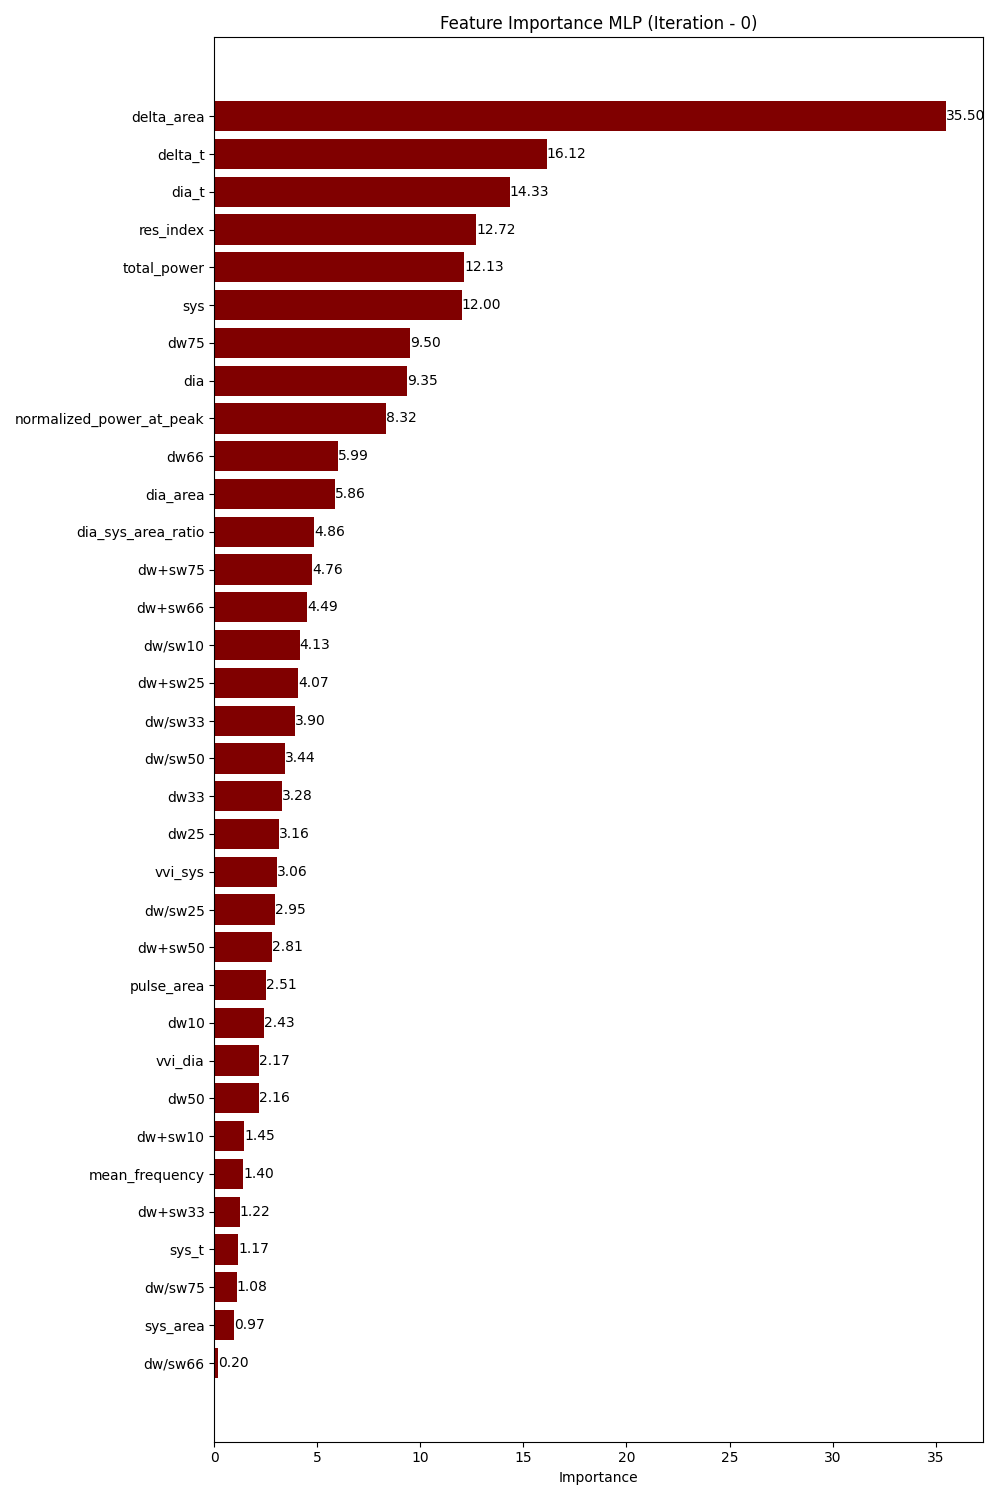
\includegraphics[width=\textwidth]{images/results/feature_importance/feature_importance_plot_MLP_0}
    \caption{Feature Importance Chart MLP}
    \label{fig:fi_mlp}
\end{figure}

\begin{figure}[h]
    \centering
    \vspace{-1cm}
    \hspace{-2cm}
    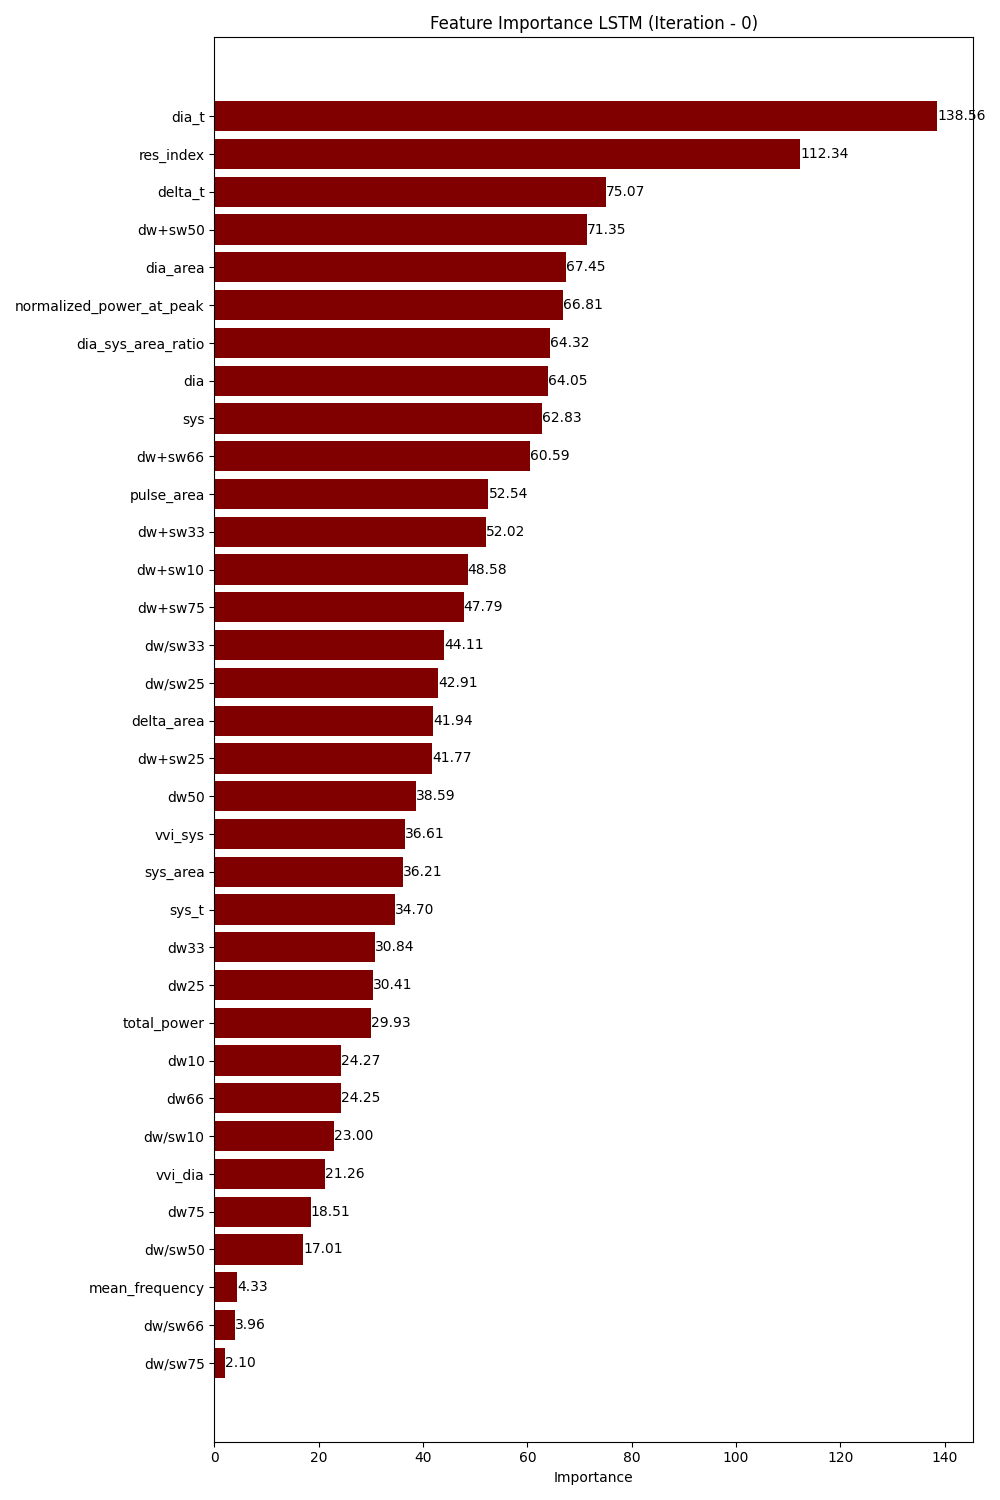
\includegraphics[width=\textwidth]{images/results/feature_importance/feature_importance_plot_LSTM_0}
    \caption{Feature Importance Chart LSTM}
    \label{fig:fi_lstm}
\end{figure}

\begin{figure}[h]
    \centering
    \vspace{-1cm}
    \hspace{-2cm}
    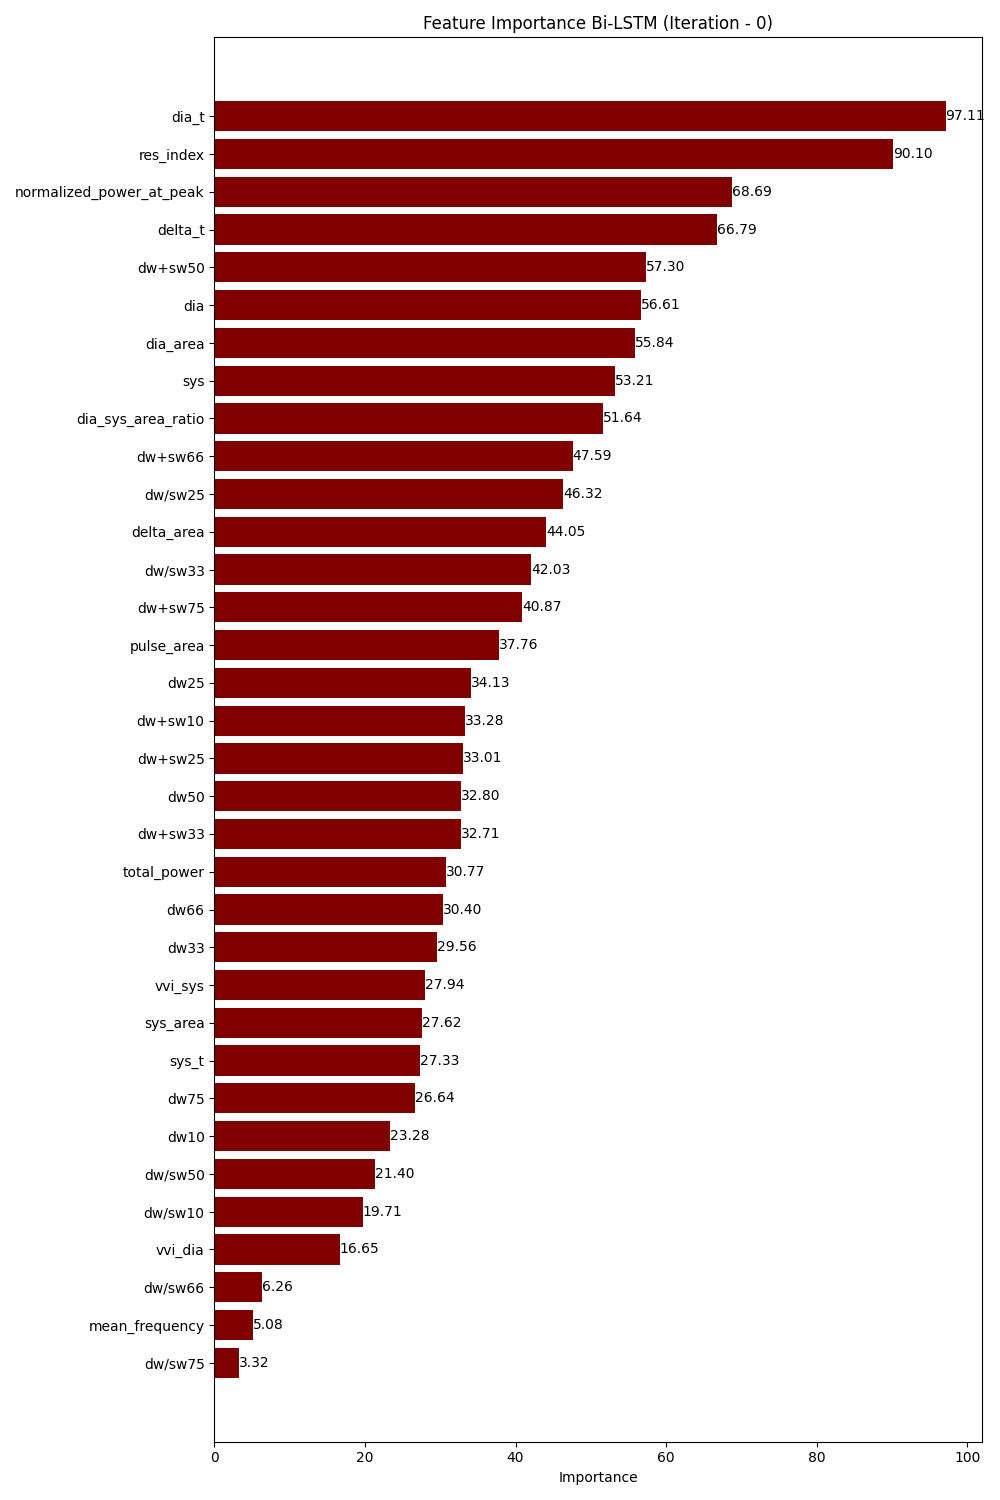
\includegraphics[width=\textwidth]{images/results/feature_importance/feature_importance_plot_Bi-LSTM_0}
    \caption{Feature Importance Chart Bi-LSTM}
    \label{fig:fi_bi_lstm}
\end{figure}

\begin{figure}[h]
    \centering
    \vspace{-1cm}
    \hspace{-2cm}
    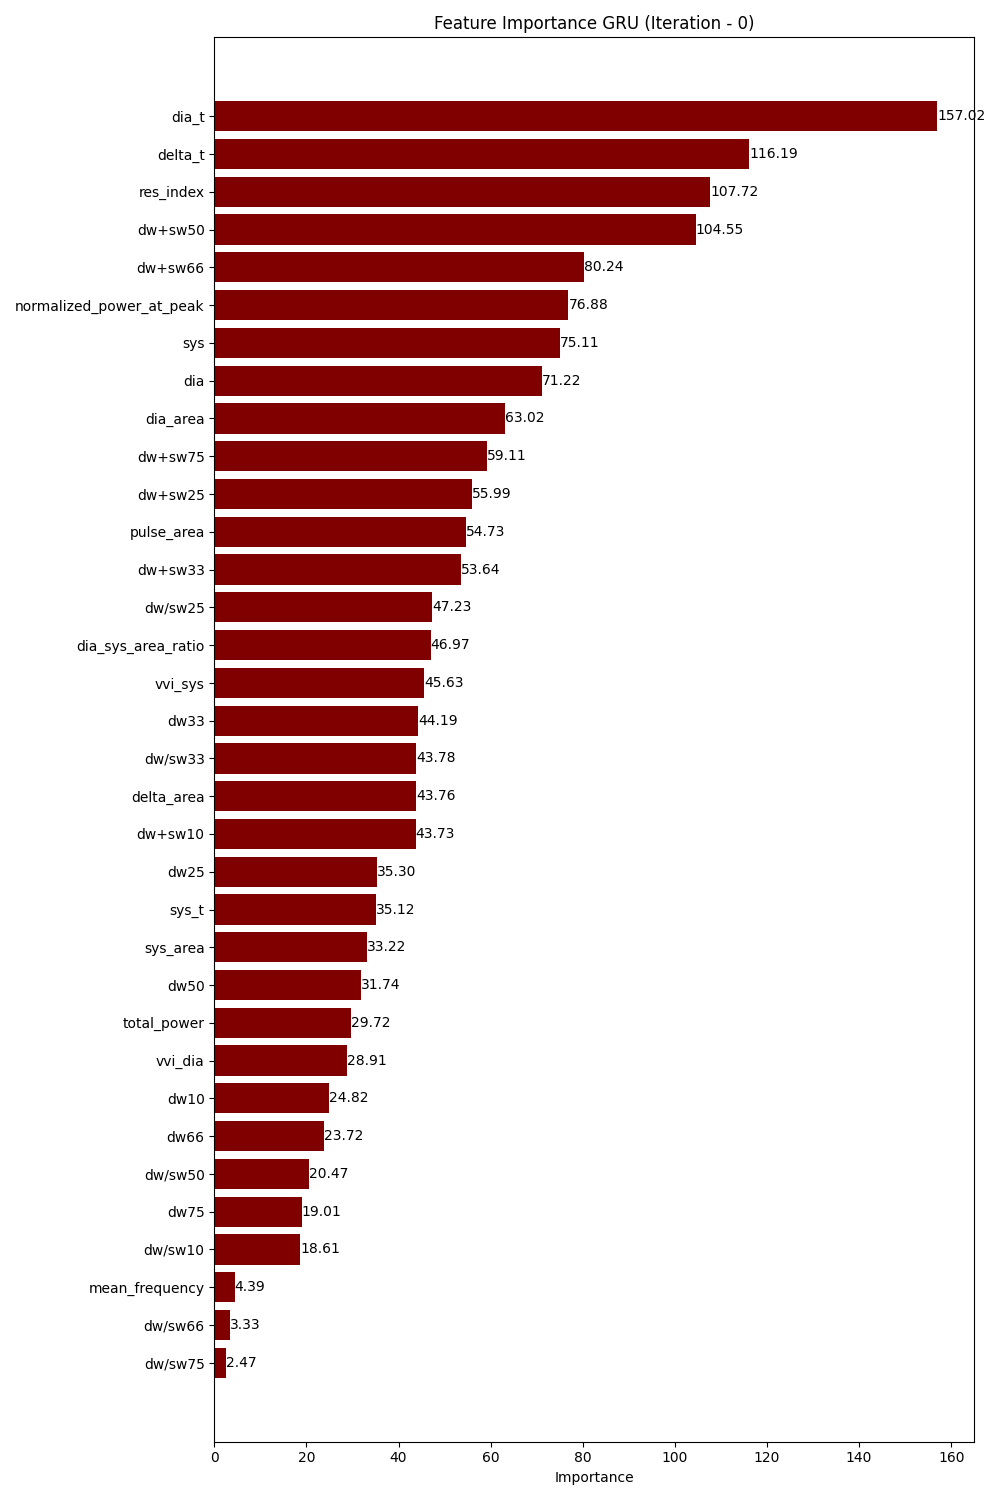
\includegraphics[width=\textwidth]{images/results/feature_importance/feature_importance_plot_GRU_0}
    \caption{Feature Importance Chart GRU}
    \label{fig:fi_gru}
\end{figure}

\begin{figure}[h]
    \centering
    \vspace{-1cm}
    \hspace{-2cm}
    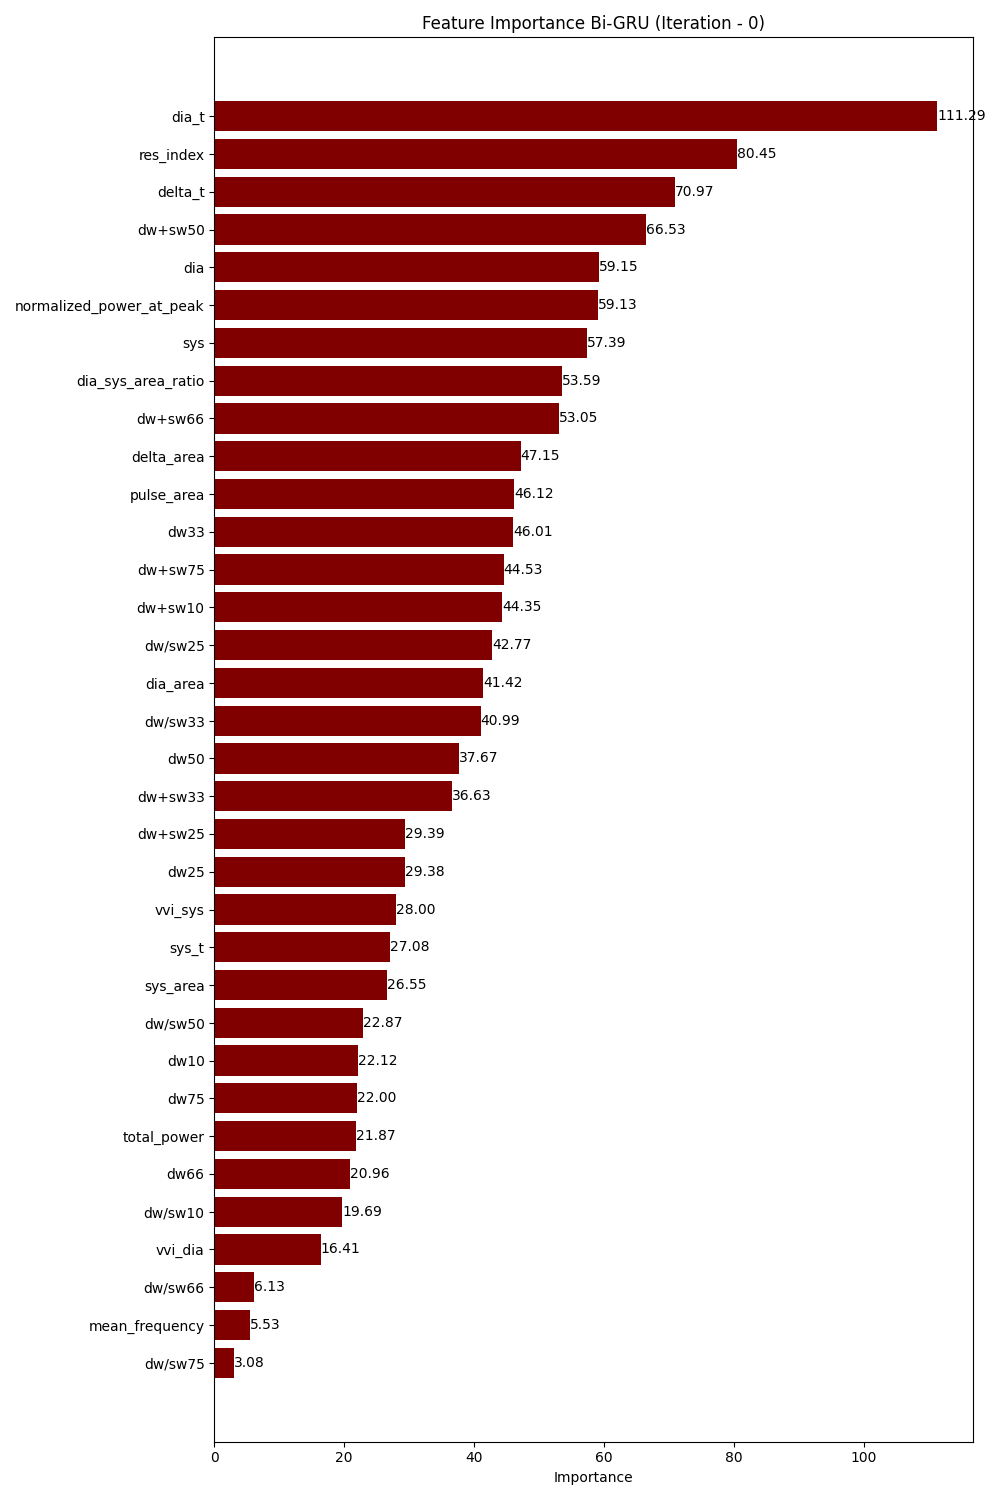
\includegraphics[width=\textwidth]{images/results/feature_importance/feature_importance_plot_Bi-GRU_0}
    \caption{Feature Importance Chart Bi-GRU}
    \label{fig:fi_bi_gru}
\end{figure}